Luonnollisesti eri sidosryhmät ovat kiinnostuneet erilaisiin käyttötarkoituksiin soveltuvista rajapinnoista. Osa sidosryhmistä on kiinnostunut vain datan lukemiseen tarkoitetusta rajapinnasta käyttäen sitä esimerkiksi käyttövarmuuden ja tuoton tilastointiin, kun taas osa on kiinnostunut järjestelmien etähallinnasta esimerkiksi verkon joustavuuden parantamiseksi. Erityyppisiä sidosryhmiä on hahmoteltu kuvassa \ref{fig:sidosryhmat}, jossa keskellä sijaitsee rajapintoja tarjoavat järjestelmät, vasemmalla sähköverkkoon liittyvät ja oikealla muut sidosryhmät.

\begin{figure}[h]
  \centering
  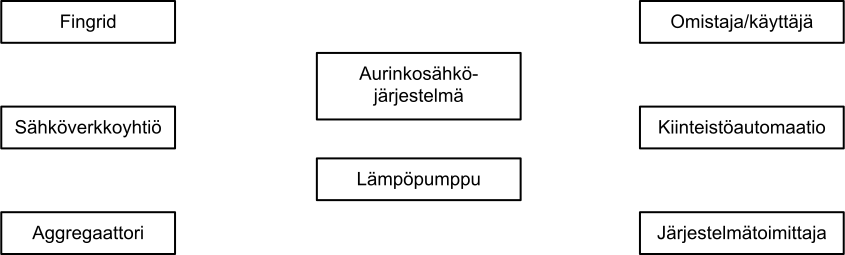
\includegraphics[width=1\textwidth]{figures/sidosryhmat}
  \caption{Järjestelmien sidosryhmiä}
  \label{fig:sidosryhmat}
\end{figure}

\section{Kantaverkkoyhtiö Fingrid}
  Suomen kantaverkkoyhtiönä Fingrid asettaa vaatimuksia siihen liittyen, mitä rajapintoja järjestelmien on sisällettävä. Se vaatii alle \SI{1}{\mega\watt} järjestelmien (voimalaitosten) sisältämään logiikkaportin, jonka kautta saapuvalla käskyllä voimalaitoksen on lopetettava pätötehon tuotanto viiden sekunnin kuluessa. Yli \SI{1}{\mega\watt}:n suuruiset järjestelmät tulee taas varustaa väyläliitännällä, jolla voidaan alentaa tuotannon pätötehoa annetun ohjearvon mukaisesti. Tämän liitännän on oltava yhteensopiva IEC60870-6, IEC60870-5 tai IEC61850 -protokollan kanssa. Fingrid ei dokumentissaan kuitenkaan ilmoita, täytyykö näiden liitäntöjen olla käytössä, vai riittääkö että järjestelmissä on liitäntä olemassa. \parencite{VJV2018}

  Mikäli Fingridin voimajohtoon liitettävä voimalaitos on yli \SI{1}{\mega\watt}:n tehoinen, se on varustettava eroonkytkentäreleistyksellä. Yli \SI{5}{\mega\watt}:n tehoinen voimalaitos vaatii lisäksi eroonkytkennän viestiyhteyden pikajälleenkytkentöjen toiminnan varmistamiseksi. Jos taas voimalaitos liittyy suoraan tai Fingridin asiakkaan verkon kautta kantaverkon kytkinkenttään, ei eroonkytkentäreleistystä vaadita. Tahattoman saarekekäytön estäminen on joissain inverttereissä integroituna, jolloin ne tarkkailevat verkon tilaa ja huomattuaan saarekkeen muodostumisen, kytkeytyvät irti. Tällöin alle \SI{5}{\mega\watt}:n järjestelmät eivät tarvitse erillisiä laitteistoja eroonkytkentään, vaan invertteri toteuttaa itsessään jo tämän vaatimuksen. \parencite{VJV2018}

  Yli \SI{1}{\mega\watt}:n järjestelmien on kyettävä joko toimimaan tehokertoimella 1.0 tai vaihtoehtoisesti tukemaan verkon jännitettä loistehoa säätämällä. Yli \SI{10}{\mega\watt}:n järjestelmien kohdalla säädön on tapahduttava automaattisesti. Lisäksi Fingridin Kantaverkkokeskus tai liittymispisteen verkonhaltija voi tarvittaessa pyytää järjestelmän käytöstä vastaavaa toimijaa muuttamaan pätö- tai loistehosäädön asetteluarvoja voimalaitosteknologian asettamissa rajoissa. Fingrid ei täten ota kantaa siihen, miten tämä säätäminen tapahtuu. Fingridin tarpeet järjestelmien rajapinnoista rajoittuvat siten erityistilanteissa järjestelmän alasajoon tai sen tehonsäätöön käytöstä vastaavan toimijan kautta. \parencite{VJV2018}

\section{Verkonhaltija}

  Yksi järjestelmien rajapintoihin liittyvistä sidosryhmistä on sähköverkonhaltija eli Suomessa sähköverkkoyhtiö. Vuodesta 2009 on Suomessa laki velvoittanut sähköverkkoyhtiöitä asentamaan sähkönkäyttöpaikoille eli pisteisiin, jossa sähköä ostavat asiakkaat liittyvät verkkoon, tuntimittauslaitteiston. Asetus myös asettaa vaatimuksia käytetyllä tuntimittauslaittestolle muun muassa etäluettavuudesta ja -ohjattavuudesta. \parencite{mittariAsetus}

  Älykkäästä tuntimittauslaitteistosta käytetään usein termiä älymittari, \gls{AMR}-mittari tai \gls{AMI}-mittari. Termin \gls{AMR} viitatessa lähinnä mittarin automaattiseen luentaan, saattaisi \gls{AMI}-mittari olla oikeampi termi. Lyhenne \gls{AMI} tarkoittaa mittareiden muodostamaa järjestelmää, jossa tieto liikkuu myös kohti mittareita ja niiden takana olevia kiinteistöjä. \parencite{dictOfEnergy}

  Verkonhaltija ei itsessään ole energian ostaja tai myyjä, vaan se siirtää sähkön verkossa ja on vastuussa verkon toimivuudesta. Tästä syystä verkonhaltijan saamat suorat hyödyt mittareiden etäohjauksesta ovat vähäiset. Yksi hyöty verkonhaltijalle on kuitenkin sähkönkäyttöpaikan irrottaminen verkosta etänä, esimerkiksi laajemman huoltotyön ajaksi. Tällöin verkonhaltijan ei tarvitse käyttää resursseja käydäkseen jokaisessa sähkönkäyttöpaikassa irrottamassa sen sähköverkosta ennen huoltotöitä. Toisaalta verkonhaltija voi tarjota palveluna AMI-rajapintaa, jolloin se voisi saada siitä tuottoa. Lisäksi, jos mittareita käytetään tehopiikkien tasoitukseen, hyödyttää tämä verkonhaltijaa, sillä tällöin verkon kapasiteetti riittää paremmin ja investointeja voidaan siirtää myöhemmälle.

\section{Järjestelmän omistaja}

  Järjestelmän omistajan eli usein käyttäjän suorittama järjestelmän monitorointi voidaan toteuttaa muutamilla eri tavoilla. Monitorointi ja ohjaus toteutetaan usein fyysisen käyttöliittymän avulla ja mikäli nämä toiminnallisuudet halutaan myös etänä, on käyttöliittymä helposti tuotavissa laitevalmistajan tarjoamaan pilvipalveluun tai mobiilisovellukseen. Mikäli valmistaja ei kuitenkaan tarjoa etämonitorointiin sovelluksia, on sellainen usein mahdollista tehdä itse, mikäli osaaminen riittää aiheeseen.

  Ongelma järjestelmän monitoroinnissa voi olla pilvipalveluiden tai mobiilisovellusten määrä, mikäli monitorointi ei tapahdu keskitetysti. Tällöin järjestelmän hallinnasta tulee loppukäyttäjälle hankalaa, jos hän joutuu tarkkailemaan montaa eri palvelua saadakseen selville järjestelmän kokonaistilan.

  Omistaja voi olla kiinnostunut myös erilaisista energiaa säästävistä ohjaustoiminnoista, hyvä esimerkki tästä on "poissa kotoa"{} \texttt{-}toiminto, jolla saadaan lämpötilaa laskettua, mikäli kiinteistö on tyhjillään pidemmän aikaa. Tämä luonnollisesti laskee myös lämmityskustannuksia.

\section{Kiinteistö}
  Kiinteistö voidaan ajatella yhtenä sidosryhmänä, joka on hyvin sidoksissa järjestelmän omistajaan.  Tämä johtuu sitä, että omistaja voi ohjata kiinteistöautomaation kautta muitakin laitteita, kuin vain lämpöpumppua tai aurinkosähköjärjestelmää. Tällöin järjestelmä voi säädellä automaattisesti kiinteistön energiatasapainoa tai siirtää varaavan lämmityksen varaaminen halvemmille tunneille.

  Kiinteistöautomaation avulla lämpöpumpun käyntijaksojen aiheuttamaa kiinteistön kuormitusta voidaan kompensoida aurinkosähköinvertterin avulla ja näin vähentää sähkönsiirron kustannuksia sekä parantaa jännitteen laatua heikoissa sähköverkoissa. Automaatiolla voidaan ajoittaa lämpöpumppujen kuormittavin jakso aurinkosähkön tuotantoaikaan, jolloin kiinteistön ottama kuorma verkosta pienenee. Tällä on kiinteistön energiakustannusten kannalta merkitystä erityisesti, jos käytössä on tehotariffi. Tällainen automaatio voi parhaassa tapauksessa mahdollistaa tehotariffissa määritellyn huipputehon pienentämisen kausittain.


\section{Järjestelmätoimittaja}

  Lämpöpumppujärjestelmän tai aurinkosähköjärjestelmän toimittaja voi hyödyntää järjestelmän rajapintoja huoltopalveluiden tarjoamiseen ja diagnostiikkaan. Seuraamalla järjestelmän toimintaa toimittaja voi ennustaa ja tilata tarvittavia huoltoja tai korjauksia, jolloin järjestelmän käyttövarmuus paranee. Tämä tuo käyttäjälle lisäarvoa ja säästöjä sekä huolettomuutta, toimittaja taas voi myydä tämän lisäpalveluna asiakkaalle. 
  
  Kuluttajan ei esimerkiksi tarvitse käyttää aikaa vikojen selvittämiseen tai huoltojen tilaamiseen. Vastaavasti toimittajan/huoltoyrityksen turhat vierailut vähenevät, kun järjestelmän virhetilanteita voidaan selvittää ja nollata etähallintaa hyödyntäen. Toimittajan suorittamaa diagnostiikkaa voidaan käyttää myös tuotekehityksen apuna tai luodessa parempia ennustemalleja sähkön kulutuksesta.

\section{Aggregaattori}

  Ennestään sähkömarkkinoilla on ollut käytännössä kolme toimijaa: Energian myyjä, siirtäjä ja ostaja. Aggregaattori näistä kaikista (mahdollisesti) erillinen toimija, jonka tehtävänä on myydä sähkömarkkinoille joustoa. Aggregaattori voi ohjata esimerkiksi lämpöpumppupoolia ja käydä kauppaa sen mahdollistamalla kysyntäjoustolla.

  Lämpöpumput ovat todennäköisesti käyttöpaikkansa suurimpia sähkönkäyttäjiä. Saksalaisessa EVU-Sperre-järjestelmässä lämpöpumppu on sähköverkonhaltijan tai muun yrityksen ohjattavissa, ja sen kuluttama energia mitataan erikseen. Korvauksena kuormanohjauksesta kuluttaja voi hyödyntää lämpöpumpputariffeja lämpöpumpun käyttämän energian hankkimiseen. Aggregaattorina toimivan yrityksen suorittama ohjaus tapahtuu AMI-mittareiden digitaalisen ohjausrajapinnan kautta. \parencite{enwg, VDEARN4100}

  Vastaavasti aurinkosähköinvertterin ohjaukseen releohjaus ei suoraan sovellu, sillä inverttereiden ohjaus tapahtuu usein monimutkaisemmalla kommunikaatiolla, kuin yksinkertaisella releellä. Sinällään tämä ei haittaa, sillä aurinkosähköjärjestelmän hyödyt etäohjauksen osalta ovat vähäiset; tavoitteena on kuitenkin saada tuotettua mahdollisimman paljon energiaa, ja tämän invertteri hoitaa automaattisesti.

  Mikäli invertterit pystyvät tuottamaan loistehoa pätötehon tuotannosta riippumatta, voi aggregaattori olla kiinnostunut ohjaamaan niitä virtuaalivoimalan tavoin isommissa ryhmissä. Nykyisillä ratkaisuilla tämä ei kuitenkaan ole vielä mahdollista. Esimerkiksi standardoitu rajapinta pilvipalveluintegraatioihin eri valmistajien välillä voisi mahdollistaa tämän, mutta ensin pitäisi varmistaa, soveltuvatko valmistajien pilvipalvelut tähän tarkoitukseen esimerkiksi tietoturvan ja käyttövarmuuden näkökulmasta.

  Aggregaattori voi myös tulevaisuudessa mahdollisesti ohjata akullisia järjestelmiä virtuaalivoimalan tavoin. Tällöin on sovittava raja-arvot, millaisilla varaustasoilla aggregaattori voi säätää energiavarastoa, jotta omistajalla on aina tarvittava vähimmäiskapasiteetti käytettävissä tarpeen tullen.
  
  Älymittareiden hyödyntäminen näihin edellä mainittuihin tarkoituksiin on tällä hetkellä haastavaa, sillä asennetuissa mittareissa ei ole muita ohjausrajapintoja kuin releohjaukset. Tulevaisuudessa mittareihin mahdollisesti tulee muitakin rajapintoja, mutta todennäköisempää on se, että aggregaattori ohjaa erillisen kiinteistöautomaation kautta kuormia. Tällöin älymittareiden käyttövarmuus ei heikenny monimutkaisten toimintojen lisääntyessä, sillä kiinteistöautomaatio sisältää monimutkaisemman kommunikaation laitteiden kanssa ja älymittari voi keskittyä mittaustiedon toimittamiseen.
